This chapter describes the design of \sys and the techniques \sys uses to
support disguising and revealing. We first look at how \sys performs disguising
transformations, and then dive into the details of how \sys reveals disguised
data.
We then describe the more complicated scenarios possible with \sys, namely disguise composition, shared
data, and action as pseudoprincipals.
This chapter concludes with an analysis of the security of \sys's design with
respect to the threat model described in \S\ref{s:threat}.

\section{\Xxing}
\label{s:applying}

To apply a \xxing transformation, \sys creates a unique \emph{\xx ID} and
queries for the data to \xx based on the \xx specification predicates.
%\lyt{Selecting all
%predicated data prior to performing database modifications ensures that
%any updates during \xxing do not affect what data to \xx. (put as footnote?
%cut? dunno)}
%
\sys then performs the specified database changes by first applying all
removals, and then decorrelations and modifications in specification order,
potentially generating and storing pseudoprincipals.
%If \sys must apply more than one change to the same selected data object
%attribute (\eg because the object satisfies multiple predicates), \sys applies
%the changes in the order specified in the spec.
%
%The developer can reason about which objects are \xxed based on the state of
%the database at the point of time the \xxing transformation occurs.
%

%
\sys next generates \emph{diff records} that contain \one{} the original data,
\two{} new placeholder data the disguise inserted or rewote in the application
(\eg pseudoprincipals or the value of any modified columns), and \three{} the
\xx ID.
%
For each new pseudoprincipal, \sys generates a public--private keypair and adds
a \emph{speaks-for record}, which adds a link to the original principal's
\emph{speaks-for chain}.
A speaks-for record contains a pair of (original principal,
pseudoprincipal) IDs and the pseudoprincipal’s
private key. \sys registers the pseudoprincipal with its public key to enable
composition of disguises (\S\ref{s:composition}).
%
\sys then encrypts the diff and speaks-for records with the principal's key,
and stores them in the database.
%
%
%
Finally, \sys returns the \xx ID to the application.
%
A client can use the \xx ID and the principal's
credentials to reveal the transformation later.
%

\begin{figure}[h]
\centering
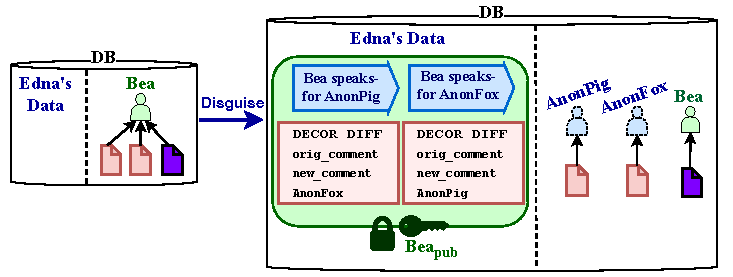
\includegraphics{figs/lobsters_catanon_visual}
\caption{When \sys applies topic-based anonymization to Bea's comments on
    stories tagged ``Star Wars'' (red), these comments are decorrelated to
    pseudoprincipals (``AnonPig'', ``AnonFox''). \sys stores encrypted
    speaks-for records mapping Bea to their
    pseudoprincipals, and diff records containing the comments with
    modified foreign keys.}
\label{f:lobsters_visual}
\end{figure}


%
To perform Bea's topic-based anonymization (Figure~\ref{f:lobsters_visual}),
\sys thus:
%
\one{} queries the database to fetch comments and votes by Bea
affiliated with ``Star Wars'';
%
\two{} creates a pseudoprincipal (\eg
``AnonFox'') for every ``Star Wars''-tagged story that Bea commented
on, and inserts it as a new user;
% into the database;
%
\three{} modifies the database by rewriting comment
foreign keys to point to the created pseudoprincipals, and
removing Bea's votes on those stories;
%
\four{} creates new speaks-for records that map Bea to the created
pseudoprincipals and create new links in Bea's speaks-for chain; diff records
containing Bea's votes on ``Star Wars'' stories; and diff records that document
Bea's original ownership of ``Star Wars''-tagged comments;
%
\five{} encrypts the speaks-for and diff records with Bea's public key, stores
them; and
%
\six{} returns a unique \xx ID to the application.

%
% \sys's security properties require that \xx records be untraceable: even a
% complete dump of \sys's state should not allow an attacker to match \xx records
% with users.
% %
% But efficient revealing requires there be a way to reference the records for a
% given \xx transformation and principal.
% %
% To this end, \sys encrypts both \xx records \emph{and} references to \xx
% records using principal public keys, which we describe next.
%
%We now describe how this works.
%

\sys adds a \emph{\xx table} and a \emph{principal table} to the application
database to store principals' \xxed data.
%
The \xx table contains lists of per-principal diff and speaks-for records encrypted with the
principal's public key.
%(Recall that private keys are not stored in the database.)
%; for instance, \verb+\xx_table[1]+ might be a list of \xx records
%pertaining to Bea's \xxing of ``Star Wars'' comments.
%
%These records are encrypted
%by Bea's public key, and thus can only be decrypted when Bea's private key is
%available.
%
The principal table is indexed by application user ID; each row contains the
principal's public key, and a list of \xx table indexes encrypted with the
public key.
%
To store records for principal $p$, \sys \one{} encrypts the records with
$p$'s public key; \two{} stores the ciphertext in the \xx table under index
\fn{idx}; \three{} encrypts \fn{idx} (salted to
prevent rainbow table attacks) with $p$'s public key; and \four{} appends the
encrypted \fn{idx} to $p$'s list of encrypted \xx tables indexes
in the principal table.
%an encrypted $[i \parallel \text{random-nonce}]$ (encrypted with the principal's public key).
%encrypts $[i \parallel \text{random-nonce}]$ with the principal's public
%key and appends the result to its principal table record.

%
This allows \sys to store records without needing access to the principal's
private key, and to do so securely: the principal table adds a layer of
indirection from user ID to encrypted records, so an attacker cannot link
principals to their records.
%
At reveal time, \sys can efficiently find \xxed data for a given user
by decrypting and using \xx table indexes in the principal table.
%
%This also hides from an attacker which \xxed data belongs to a given principal
%because entries in the principal table cannot be interpreted without
%principals' private keys, which are not stored in the database.
%

%
\Xxing transformations may completely remove a principal from the
application database.
%
When this happens, \sys moves the corresponding list of encrypted \xx table
indexes from the principal table to a \emph{deleted principal table} indexed
opaquely, \eg by the public key.
%
This removes the user ID from the database while allowing future reveal
operations by the principal to find their \xx table indexes.
%

%%%%%%%%%%%%%%%%%%%%%%%%%%%%%%%%%%%%%%%%%%%%%%%%%%%%%
\section{Revealing}
\label{s:reveal}

%
To apply a reveal transformation, \sys first locates and decrypts the
corresponding diff and speaks-for records using a \xx ID and the user’s reveal
credentials.
%

\begin{figure}[t]
  \small
\begin{lstlisting}[style=pseudo,escapeinside={(*}{*)}]
Reveal(disgID, uid, privkey):
 encrypted_disg_table_idxs := principal_table[uid]
 decrypted_disg_table_idxs :=
    decrypt(encrypted_disg_table_idxs, privkey)
 for idx in decrypted_disg_table_idxs:
   records = decrypt(disg_table[idx], privkey)
   for rec in records:
     if rec.disgID == disgID:
       // apply rec to application database
       // remove rec from disg_table
     else if rec.type == SPEAKS_FOR:
       // recursively reveal for pseudoprincipal
       // generated by another disguise
       Reveal(disgID, rec.pp_uid, rec.pp_privkey)
\end{lstlisting}
    \caption{Pseudocode for revealing a \xxing transformation while
    application principal \fn{uid} exists. Recursive revealing (the
    \texttt{\small else} clause) walks the speaks-for chain to reveal composed
    records of pseudoprincipals created by other disguising transformations
    if necessary (\S\ref{s:composition}).}
  \label{f:revealpseudo}
\end{figure}

\sys's reveal procedure (Figure~\ref{f:revealpseudo}) first looks up all \xx
records related to the provided reveal credentials via \sys's principal and \xx
tables.
%
\sys then applies diff records created for the \verb+disgID+ \xx transformation
to the database, thus restoring the relevant
application objects to their pre-\xxed state.
% Additionally, \sys recursively applies the procedure for
% pseudoprincipals that the current user speaks-for; this supports the
% composition of \xxing transformations, such as a Lobsters user who removes
% their previously-anonymized contributions (\S\ref{s:composition}).

%
To preserve referential integrity, \sys first restores \xxed data that was
removed.
%
\sys then reveals any modifications, and finally performs recorrelations. 
%using decrypted speaks-for records.
%
Finally, \sys de-registers any pseudoprincipal who no longer has any associated
disguised data, removing them from the principal table and the application's
users table.
%
Developers can configure \sys to also check for references to pseudoprincipals
prior to removing them, and depending on the application's needs, configure \sys
to delete, rewrite, or leave the references in place.
%
After revealing, the \xxed data is no longer needed, so \sys clears the
corresponding diff and speaks-for records.
%

%
In the example, if Bea wants to reveal their ``Star Wars'' contributions,
Lobsters invokes \sys with the \xx ID and Bea's password as reveal credentials.
%to reveal their Star Wars \xxing transformation.
%
\sys uses the password to reconstruct Bea's private key, retrieve and decrypt
Bea's records, and filter those records for those with the \xx ID.
%
\sys then restores deleted votes and Bea's ownership of
decorrelated comments.
%

\subsection{Revealing in the Presence of Application Updates}

\begin{figure}[h]
\centering
    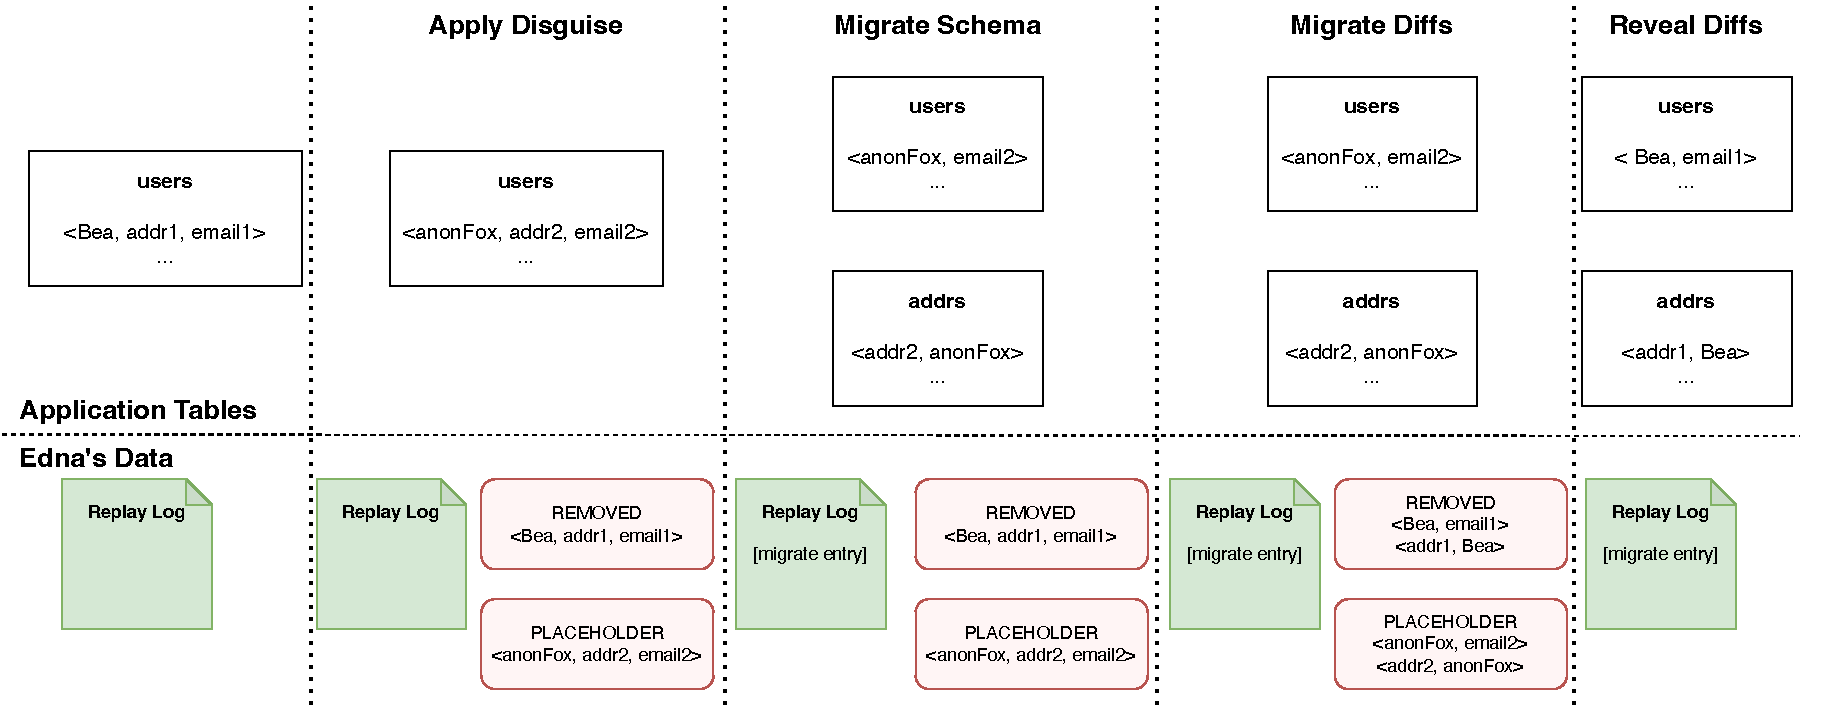
\includegraphics[width=\textwidth]{figs/updates}
\caption{When the application applies updates like schema migrations, it can
    invoke \sys to log the migration, which then is applied to disguised data in
    diff records prior to reveal.}
\label{f:updates}
\end{figure}



\sys's revealing as described thus far may accidentally reveal data that ignores
database changes applied since the time of disguise, such as application updates
to un\xxed data or schema migrations.
%
To prevent this, \sys utilizes developer-provided information about important
updates and schema migrations to apply them to \xxed data prior to revealing it,
ensuring that revealed data reflects the current state of the database.
%
Prior to revealing the udpated data, \sys will also perform consistency checks
to guarantee adherence to internal database invariants, such as uniqueness
constraints.
%
Here, we describe how developers specify application updates and schema
migrations; how \sys applies these updates to data to reveal; and \sys's
consistency checks.

%
\subsubsection{Applying Application Updates}
In order for revealing to preserve application correctness, \sys must know about
application updates that alter application invariants.
%
Consider an example where a moderator periodically edits all posts to remove
swear words, creating an implicit invariant that all posts created prior to the
last moderation pass should contain no swear words.
%
If a user's disguise removes their posts, then a moderation pass occurs, and
then the user wants to restore their posts, \sys would not know about these
moderation updates to posts of the application and incorrectly restore the
original post content with swear words present upon reveal.
%
However, \sys could correctly restore the post if it knew to remove the swear
words prior to reveal.
%
%Likewise, if \sys removed the post instead of scrubbing its content, the
%moderator would never see it (and could not edit it), but \sys would reveal the
%post with swear words still present.
%
%In the first scenario, \sys knows that an update was applied, and refuses to
%reveal the modified post; in the second, \sys does \emph{not} know that
%moderation happened and reveals the removed post.
%%
%Neither might be what the application desires.
%

\sys handles this situation by tracking applied application updates in a
\emph{replay log} of application updates.
%
The application invokes \sys when it performs operations that need to hold
over revealed data---\eg moderations---and \sys records these updates in its replay
log.
%
When revealing data, \sys applies, in order, every entry in the replay log
added since the time of disguise to the disguise's diff records.  
%

%
Log entries map the original data and the new placeholder data in diff records
to corresponding updated-original and updated-placeholder data. 
%
After applying all updates to placeholder data, \sys takes the
updated-placeholder data and removes it from the database.
%
Similarly, after applying all updates to the original data, \sys takes the
updated-original data and restores it to the database.

%
In the swear words moderation example, \sys queries the replay log, sees
the swear words moderation entry, and then applies the swear words moderation to
the removed post data in the diff record. (Note that in this example, the diff
record contains no new placeholder data that replaced the removed post; in other
scenarios such as decorrelation or modification, \sys would apply the logged
update to new placeholder data as well). Only then does \sys restore the post
with no swear words (and had new placeholder data existed, \sys would remove the
updated placeholder data).
\lyt{Too confusing?}

\subsubsection{Applying Schema Migrations}
Applications also constantly undergo schema migrations to reorganize data or add
new application features. When these occur, \sys must know how to manipulate any
disguised data structured in the old database layout to match that of the
current database.
%
\sys allows applications to invoke \sys with a replay log entry encoding the
schema migration after the migration is performed.
%
As with application updates, schema migration entries map diff record data to
migrated-original data and migrated-placeholder data, which \sys then
respectively restores and removes.

For example, as shown in Figure~\ref{f:updates}, a developer of an application
with a \texttt{users} table that contains rows with \texttt{username}s,
\texttt{addr}s, and \texttt{email}s may choose to allow users multiple
addresses.  They would create a new \texttt{addrs} table, with a foreign key to
the users table, and populate \texttt{addrs} using the address data in
\texttt{users}.  Finally, they would remove the \texttt{addr} column from
\texttt{users}.
%
The corresponding replay log entry would map an original \texttt{users} data row
in a diff record to both a row in \texttt{users} with username \texttt{uid} and
a row in \texttt{addrs} that has a foreign key of \texttt{uid} to
\texttt{users}. These rows would be restored to the database.
%
It would also generate two rows for any placeholder \texttt{users} data row in a
diff record and remove these from the database.
%

\subsubsection{Consistency Checks for Internal Invariants} 
After applying any developer-specified migrations or updates since the time of
disguising, \sys still needs to perform consistency checks on the data to reveal
to ensure that revealing will not violate the database's integrity.
%
These checks only allow revealing if the revealed data: \one{} will still
satisfy uniqueness and primary key constraints; \two{} will not overwrite
modifications that occurred while data was \xxed; and \three{} will maintain
referential integrity.

For \one{}, \sys checks that \emph{removed} \xxed data is still removed from the
database;
%
and for \two{}, \sys ensures that \emph{modified} \xxed data is in the same
modified state and \emph{decorrelated} \xxed data is still affiliated with the
same pseudoprincipal in the database using the new value stored in the diff
record.
%
To ensure \three{}, \sys checks for the existence of all objects referenced by
the data to reveal (\eg a post referenced by a to-be-revealed comment).
%and ensures that any foreign key references to pseudoprincipals to be deleted
%are rewritten to the original.

\sys is conservative and will never reveal rows for which checks fail; the
affected data remains \xxed.  For example, if a developer chooses not to
register conflicting application updates or schema migrations, \sys's checks may
fail, preventing disguised data from being revealed.
%
\sys could flag encountered conflicts, giving the application a chance to fix
them so a later reveal can pass the checks.

\subsubsection{Limitations}
\label{s:design:updates:limitations}
\sys's replay log approach faces some limitations. First, it assumes that either
\one{} updates applied to a row rely on at most that row's data, and not the
data of other disguised rows or external database state; or \two{} that any
external dependencies of an update will not violate application invariants or
expose which data had been disguised.
%
For example, take an update that calculates the current vote count of a post to store
as a post's \texttt{vote\_count} attribute, and say that 
a disguise has removed both a user's post and its votes.
%
When \sys reveals the disguise, \sys will first reveal the diff records for
posts before revealing those for votes in order to maintain referential
integrity. But when applying the \texttt{vote\_count} update to post diff
records, \sys will find 0 votes for the post, because the votes have not yet
been restored.
%
One potential solution would be for developers to indicate the data dependencies
of each update, so \sys could know to restore votes before posts; however, this
requires \sys to disable foreign key checks and carefully check for referential
integrity after restoring posts, since restoring votes first can now
inadvertently leave dangling pointers. Or perhaps developers could schedule cron
jobs to habitually perform the update to ``fix up'' any rows that have been
revealed since the update; however, this only works for an idempotent update, as
it should not modify already-modified rows again.
%

%
Furthermore, developers must do additional work to add hooks to invoke \sys when
any major application change or schema migration occurs. Invoking these hooks
and applying these updates during reveal also adds additional computation work;
we measure these costs in \S\ref{s:eval:updates}.
%
Finally, replay logs only apply to diff records, which contain the actual data
changes, and not speaks-for records; \sys assumes that the identifiers for
principals in speaks-for records that encode the speaks-for chain remain
consistent as the database changes.
%

%%%%%%%%%%%%%%%%%%%%%%%%%%%%%%%%%%%%%%%%%%%%%%%%%%%%%%%%%%%%%%%%%
\section{Shared Data}
\label{s:shared}
%
Many applications support shared data; in Lobsters, for example, messages
between users are owned by both users.
%or co-authored papers in HotCRP.
%
\sys's default semantics for shared data implement an ownership model inspired
by a common treatment of messages as jointly owned.
%
When a user \xxs shared data, \sys decorrelates the data from the \xxing user,
but preserves the data and its association with other owners.
%
\sys removes the data once all users have \xxed it and all ownership links are
to pseudoprincipals.
%
For instance, consider a Lobsters message between Bea and Chris: after Bea \xxs
the message, the message is owned by Chris and a pseudoprincipal; if Chris then
\xxs the message, \sys removes it.
%
Either owner can reveal the message, which restores the message to the database
and recorrelates the revealing user; the other owner remains decorrelated as a
pseudoprincipal until they also choose to reveal the message.
%
Regardless of the reveal order, if all owners reveal the message, \sys returns
the message to its original state.
%

%%%%%%%%%%%%%%%%%%%%%%%%%%%%%%%%%%%%%%%%%%%%%%%%%%%%%%%%%%%%%%%%%

%%%%%%%%%%%%%%%%%%%%%%%%%%%%%%%%%%%%%%%%%%%%%%%%%%%%%%%%%%%%%%
\section{Composing \Xxing Transformations}
\label{s:composition}
\todo{Figure? Check for clarity of OOO reveals and SFC}

\begin{figure}[h]
    \centering
    \small
    \begin{tabular}{c|c|c|c} %|m{0.08\linewidth}}
        Operation & Remove & Modify & Decorrelate \\
        \hline
        Remove & $\varnothing$ & $\varnothing$ & $\varnothing$\\ 
        \hline
        Modify & Remove data & Modify data & Decorrelate data\\ 
        \hline
        Decorrelate & Remove data$^*$ & Modify data$^*$ & Recursively decorrelate data$^*$\\ 
    \end{tabular}
    \caption{What happens when disguise operations compose, with the first
    operation on the vertical, and the second operation on the horizontal. $^*$
    represents operations that require special handling, using the user's reveal
    credentials to find previously-decorrelated data to disguise and recursively
    disguise them.}
    \label{tab:composition}
\end{figure}

\sys supports composition of \xxing transformations, which occurs when a
transformation applies to data that \sys had previously \xxed in
some other way.
%
Reasoning about composition of transformations can be broken down to reasoning
about the composition of primitive operation pairs, \eg remove after
modify, or remove after decorrelation.
%
Many pairs result in trivial composition: no operation can be composed after a
remove (the data is gone), and any operation after a modify updates the
data as expected. %Revealing these pairs in any order

However, operations after decorrelation results in more complex composition scenarios.
%
For instance, decorrelation after decorrelation could occur if a user
decorrelates some posts, after which an administrator decorrelates \emph{all}
posts. In this scenario, the administrator's \xxing operation applies to
pseudoprincipal-owned posts in the same way as it does to unmodified posts. This
creates pseudoprincipals that can speak-for other pseudoprincipals.  \sys uses
the pseudoprincipal's registered public key to encrypt pseudoprincipal diff and
speaks-for records, so \sys does not need to know its link to an original
principal in order to encrypt and \xx its data.
%

%
%For instance, a user could decorrelate their posts, after which an
%administrator could modify all posts (including those of pseudoprincipals) by
%removing associated metadata.
%

%Another interesting case is when a transformation should apply to data that a
%user owned, but that has already been decorrelated.
Removal or modification after decorrelation also require special handling. For
instance, a Lobsters user might first decorrelate some of their comments and
then request to delete all their comments (\eg by deleting their account).
%
But the decorrelated comments are no
longer linked to the original user; how can the deletion transformation find
them?
%
\begin{comment}
%\sys by default handles \xxing of previously modified or decorrelated data
%without any problems: pseudoprincipals have affiliated public keys, and \sys
%treats them the same as any other principal when \eg an administrator wants to
%\xx all users' posts.
%
%Users can reveal \xxed data on behalf of their pseudoprincipals as described in
%\S\ref{s:reveal}.
\end{comment}
%
\sys addresses this question by accepting optional reveal credentials as part of
the \xx operation.
%
These credentials let \sys decrypt the user's previous diff and speaks-for
records, find all pseudoprincipals corresponding to that user, and apply \xxing
transformations on behalf of those pseudoprincipals as well as the user.
%
\sys uses pseudoprincipal private keys in decrypted speaks-for records as
credentials to recursively find pseudoprincipals from multiple decorrelations.

%
%\begin{comment}
%This lets \sys support Lobsters users first decorrelating their data, and then
%removing (or modifying) it via an additional \xxing transformations applied
%with their reveal credentials.
%\end{comment}
%\lyt{Without reveal credentials, \sys would not \xx any of the
%user's data previously decorrelated to pseudoprincipals.}
%and include them in the query to the application database.
%

\subsection{Out-of-Order Reveals}
\label{s:design:oooreveals}
\todo{check}
\sys must also handle reveals of transformations in any order.  As before,
many scenarios are straightforward: revealing removals is trivial (data can
only be removed and restored once), and revealing modified data simply restores
the original (subject to consistency checks).
%
Handling out-of-order reveals of multiple decorrelations presents the
greatest challenge.
%
\sys's semantics enforce that data that is decorrelated multiple times will not
be recorrelated until all \xxs are removed.
%also enables another desirable form of
%\xxing composition: .
%One desirable form of \xxing composition required special support:
%
For example, if Bea separately decorrelates their comments on ``bears''
and ``Star Wars'' posts, then later reveals the ``bears'' posts, they might want
Ewok-related comments (tagged both ``Star Wars'' and ``bears'') to remain
\xxed, even though they were initially \xxed under the ``bears'' transformation.
%
%To realize this, \sys lets a \xxing transformation recursively operate over
%pseudoprincipals' data when their \emph{owner} (authorized through credentials
%that let them access a speaks-for record) invokes it.
%
%With reveal credentials, \sys finds pseudoprincipals with
%already-decorrelated comments and applies the \xxing transformation to these
%pseudoprincipals. This again creates pseudoprincipals that can speak-for other
%pseudoprincipals.
%
To support this, \sys maintains a chain of speaks-for records that represent
speaks-for relationships between pseudoprincipals.
%
All reveal operations walk the full speaks-for chain to reveal
all necessary records (cf.\ Figure~\ref{f:revealpseudo}).

Furthermore, if reveal operations perform recorrelations out of order, \sys
removes an intermediate link in the speaks-for chain.
%
To describe how this works, take the example of two disguises that decorrelate
comments on ``bears'' and ``Star Wars'' posts respectively. The ``bears''
decorrelation rewrites Ewok posts to pseudoprincipal $P_1$; and the ``Star
Wars'' decorrelation composed on top decorrelates Ewok posts from $P_1$ to
pseudoprincipal $P_2$.  At this point, \sys has speaks-for records for Bea that
encode a speaks-for chain from Bea$ \to P_1 \to P_2$.
%

If Bea first reveals the ``bears'' anonymization---the first applied
disguise---on their data, \sys finds all accessible speaks-for records given
Bea's reveal credentials (cf.\ Figure~\ref{f:reveal-pseudo}), and constructs Bea's
speaks-for chain as a graph of principal-to-principal edges (namely Bea$\to
P_1\to P_2$).
%
\sys finds that $P_1$'s ``Ewok'' posts no longer exist in the database (they belong to
$P_2$ due to the composed ``Star Wars'' disguise), and thus does not restore 
``Ewok'' posts to Bea. \sys does still remove pseudoprincipal $P_1$ in the process
of restoring ``bear'' diff records, and once done, clears all ``bear'' 'diff
records from its encrypted disguise table. 
%
Importantly, however, \sys still retains the speaks-for record for Bea$\to P_1$,
since $P_1$ still has associated disguised data (namely a speaks-for record to $P_2$)!
%

%
Now, if Bea reveals the second applied disguise---``Star Wars''---\sys
finds diff records for decorrelated ``Ewok'' posts whose original rows have $P_1$ as
owner. 
%
However, \sys cannot reveal the diff record directly and restore the
decorrelated posts to $P_1$, as this will fail referential integrity consistency
checks, and also result in incorrect composition semantics. Instead, \sys checks
the speaks-for chain (Bea$\to P_1 \to P_2$) to determine the \emph{next valid}
user in the chain who speaks-for $P_2$, which in this case is Bea.
%
Validity is determined by whether the user is a natural principal or a
pseudoprincipal yet to be recorrelated. If a pseudoprincipal has a decorrelate
diff record from any disguise still present in Bea's disguised data, \sys knows
the pseudoprincipal has not yet been recorrelated.
%

%
After determining Bea is the next valid user in the speaks-for chain to $P_2$,
\sys rewrites the ``Ewok`` diff record to reference Bea instead of $P_1$,
and then restores the diff record like normal.
%
Finally, \sys deletes the diff records for the ``Star Wars'' disguise, the
speaks-for records for $P_2$ (which no longer has any associated disguised
data), and the speaks-for records for $P_1$ (which also has no associated
disguised data after $P_2$ is removed).
%
This implicitly truncates the speaks-for chain to simply be Bea.
%
%This design works even in the presence of multiple recursive decorrelations and
%many-link speaks-for chains. 
In general, \sys enforces the invariant that the chain only truncates at link
$L$ once all pseudoprincipals recursively generated in the chain beyond $L$ have
been recorrelated.
%

%%%%%%%%%%%%%%%%%%%%%%%%%%%%%%%%%%%%%%%%%%%%%%%%%%%%%%%%%%%%%%%%%%%%%%%%

%
%(in which case,
%an earlier link in the speaks-for chain may be removed).
%Pseudoprincipal-to-pseudoprincipal speaks-for relationships requires special
%handling during reveal operations: \sys %which must ensure that chains of speaks-for records remain linked to the
%original user even if reveal operations are applied out of order.

\begin{comment}

    To prevent such revealing behaviors, the user must provide their reveal
    credentials to tell \sys which pseudoprincipals the user can speak-for and
    whose data the user can recursively \xx.
%
    If Lobsters requires Bea to provide their reveal credentials when \xxing
    ``sci-fi'', \sys can then use those credentials to get Bea's speaks-for
    records, which relate Bea to any pseudoprincipal created for their ``Star
    Wars'' content.
%
    Equipped with the knowledge of these pseudoprincipals, \sys can now find
    comments that have the ``sci-fi'' tag \emph{even if} they also have the
    ``Star Wars'' tag (and thus have been already decorrelated).
%
    \sys then recursively decorrelates these dually-tagged comments from Bea's
    existing pseudoprincipals.
    %Rather than create a speaks-for record from \emph{Bea} to a new
    %pseudoprincipal , for these comments, \sys creates speaks-for records from
    %$p$ to $q$.
%

%
    Recursive decorrelation creates a chain of speaks-for records in \sys that
    ensures correct behavior on revealing.
%
    If Bea reveals their ``sci-fi'' comments first, the comments simply revert
    to being owned by Bea's pseudoprincipals.
%
    If Bea reveals their ``Star Wars'' comments first, \sys detects that
    dually-tagged comments are associated with another layer of pseudoprincipals
    in the application database, and does not reassociate them; instead, \sys
    simply
    %since the ``sci-fi'' \xxing transformation decorrelated the comment yet
    %again.
%
    %Comments with both tags continue to be owned by $q$, because \sys's reveal
    %process leaves modifications to the application database in place if they
    %happened after \sys applied the transformation it is currently revealing.
%
    internally updates the chain of speaks-for records so that only one layer of
    pseudoprincipals remain.

%
%
    %If Bea chooses to reveal the second transformation, \sys in both cases
    %reveals the original content, without having incorrectly revealed
    %``sci-fi'' comments in the intermediate state.
%
    %This composition is not a concern for votes, since the ``Star Wars''
    %\xxing transformation already removed them from application database.
%

%Lobsters expects that all ``sci-fi'' content decorrelated via category-based
%anonymization will remain decorrelated until Bea

\iffalse
% OUTLINE
% - introduce how pseudoprincipals are dealt with in the system
%    - have own keypair that is encrypted (chaining works)
%    - can own bags
%    - (encrypted) locators are kept as part of metadata for pseudoprincipald
% - process of chaining two \xxings
%       - go over steps in diagram (using example)
% - process of shared data
%       - use example of private messages here
An application may let a principal apply multiple \xxing transformations, some
of which may \xx data decorrelated to pseudoprincipals by some prior
transformation.
%
If data decorrelated by \xxing transformation $s$ could never be \xxed again,
then re-correlating the data by revealing $s$ might prematurely reveal data
\xxed by transformations applied after $s$.
%

\head{Composing Decorrelations.}
%
To solve this, \sys lets users \xx the data of pseudoprincipals that they can
speak-for.
%
This introduces a layer of indirection, so that revealing either transformation
will leave the decorrelating effects of the other in place.
%
To realize this indirection, \sys lets a \xxing transformation recursively
operate over pseudoprincipals' data when their \emph{owner} (authorized
through credentials that let them access a speaks-for record) invokes it.
%

%
In the example, \sys has access to Bea's reveal credentials when applying the
second \xxing transformation, so \sys can use those credentials to inspect any
of Bea's already-\xxed data.
%
This includes speaks-for records, which relate Bea to any pseudoprincipal $p$
created for their ``Star Wars'' content.
%
Equipped with the knowledge of these pseudoprincipals, \sys can now find
comments that have the ``sci-fi'' tag \emph{even if} they also have the ``Star
Wars'' tag (and thus have been already decorrelated).
%

%
Rather than create a speaks-for record from Bea to some new pseudoprincipal $q$
for these comments, \sys creates speaks-for records from $p$ to $q$.
%
This creates a chain of speaks-for records (Bea speaks-for $p$, which
speaks-for $q$) that ensures correct behavior on revealing.
%
If Bea reveals their ``sci-fi'' comments first, the comments simply revert to
being owned by $p$.
%
If Bea reveals their ``Star Wars'' comments first, \sys detects that these
comments are now owned by $q$ in the application database, since the ``sci-fi''
\xxing transformation changed the owner from $p$ to $q$.
%
Comments with both tags continue to be owned by $q$, because \sys's reveal
process leaves modifications to the application database in place if they
happened after \sys applied the transformation it is currently revealing.
%
\sys internally removes the mapping from Bea to $p$, and instead maps
Bea directly to $q$.
%
If Bea chooses to reveal the second transformation, \sys in both cases
reveals the original content, without having incorrectly revealed ``sci-fi''
comments in the intermediate state.
%

% --------------------------------------------------------------------------------

% Application of a new \xxing transformation $s_2$ on data \xxed
% by $s_1$ is relatively straightforward if $s_1$ only modified the data:
% %
% \sys encrypts stored records from $s_2$ with the associated principal’s public
% key, allowing that principal’s client to reveal the \xxing transformation by
% providing the corresponding private key. (\Xxing over data removed by $s_1$ is
% impossible because the data does not exist.)
% %
% However, if $s_1$ decorrelated data and reassociated it with pseudoprincipals,
% then $s_2$ cannot find the associated principal or its public key.
% %
% To solve this, \sys creates public/private keypairs for pseudoprincipals,
% encrypts pseudoprincipal data with pseudoprincipals' public keys, and lets a
% natural principal prove a speaks-for relationship with these pseudoprincipals.

% \lyt{Not sure if this is the right place...}
% In the following, we refer to all encrypted data that \sys produces when
% applying \xxing transformation $s$ as a \emph{bag}; locator \lcapa{ps} points
% to the bag of principal $p$'s \xxed data produced when applying $s$.

% %%%%%%%%%%%%%%%%%%%%%%%%%%%%%%%%%%%%%%%%%%%%%%%%%%%%%%%%%%
% \head{Storing Data for Pseudoprincipals.}
% %
% Each time \sys creates a new pseudoprincipal $q$ for natural principal $p$
% during $s_1$ (with $p$'s public key still available), it generates a keypair
% for $q$.
% %
% \sys then ``wraps'' $q$'s private key by encrypting it with $p$'s public key,
%  stores it with records created by $s_1$ at locator \lcapa{ps_1}, and
% forgets the plaintext private key.
% %stores it at bag pointed to by locator \lcapa{ps_1}, and
% %
% Hence, access to $q$'s private key---or records encrypted for $q$---requires $p$'s private key.
% %
% \sys then stores $q$'s public key via \fn{RegisterPrincipal} and uses it to encrypt $q$'s records.
% %
% This idea applies recursively: in the above example, $p$ itself may
% be a pseudoprincipal and not a natural principal.
% %
% (This is why the application cannot \eg simply email $q$'s private key to
% $p$ when it creates a pseudoprincipal $q$.)
% %
% In this case, \sys encrypts $q$'s private key with the public key of
% pseudoprincipal $p$, granting any natural principal who can access
% $p$'s private key access to $q$ and its data.
% %
% Thus, the bag at locator \lcapa{ps} contains both $p$'s encrypted records and
% pseudoprincipal private keys from \xxing transformation $s$.

% %%%%%%%%%%%%%%%%%%%%%%%%%%%%%%%%%%%%%%%%%%%%%%%%%%%%%%%%%%%
% \head{Pseudoprincipal Metadata.}
% %
% When $s_2$ creates a record bag encrypted for pseudoprincipal $q$, it produces
% locator \lcapa{qs_2} for the bag.
% %
% \sys stores this locator with pseudoprincipal $q$'s metadata, but encrypts
% it with $q$'s public key.
% %
% Encrypting pseudoprincipal locators ensures that \sys never exposes the mapping
% from a principal to its locators once a principal has \xxed their account (\sys
% returns all locators of natural principals to the application when \xxing, as
% described in \S\ref{s:design:\xxing}).
% %
% Locator \lcapa{qs_2} will only be needed to reveal $s_2$---and at that point,
% $q$'s private key will be available, as the principal who speaks-for $q$
% unwraps it.
% %

% %
% As an optimization, the application can tell \sys to return \lcapa{qs_2} instead
% of storing it; the application is then responsible to return the locator to
% the correct natural principal (\eg displaying a QR code to a client invoking $s_2$).
% %
% %$p$'s private key and bag locator \lcapa{ps_1} are available.
% %This causes \sys to return pseudoprincipal bag locators without
% This avoids an extra encryption per pseudoprincipal.
% %
% $p$ then reintroduces these locators when they reveal $s_2$.
% %

% \begin{figure}[t]
%     \centering
%     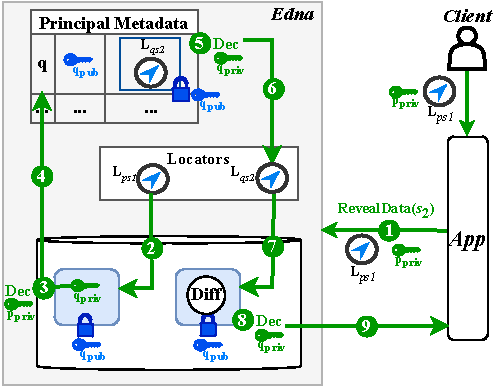
\includegraphics{figs/edna_reveal}
%     \caption{To retrieve diffs from composed \xxing transformation $s_2$, \sys
%              first decrypts $q$'s private key in $p$'s bag for $s_1$,
%              and uses that private key to decrypt \lcapa{qs_2} and the bag
%              it points to.}
%     \label{f:recursive}
% \end{figure}

% \newcommand*\circled[1]{\tikz[baseline=(char.base)]{
%             \node[shape=circle,draw,inner sep=1pt] (char) {#1};}}
% %
% Figure~\ref{f:recursive} shows how a natural principal reveals a composed
% \xxing transformation. %using the low-level API.
% %
% \lyt{(Added the following:)} In this example, clients provide private keys as reveal credentials.
% %
% \circled{1} The application asks \sys to reveal $s_2$ using $p$'s
% private key and \lcapa{ps_1}.
% %
% \circled{2}
% \sys looks up \lcapa{ps_1} to find $p$'s bag for $s_1$, and \circled{3}
% decrypts it with $p$'s private key.
% %
% This reveals that $s_1$ created pseudoprincipal $q$ and reveals $q$'s private
% key, so \circled{4} \sys looks up $q$'s metadata and
% \circled{5} decrypts $q$'s locators with $q$'s private key.
% %
% \circled{6} This provides \sys with \lcapa{qs_2}, so it \circled{7} looks
% up $q$'s bag for $s_2$, \circled{8} decrypts it with $q$'s private key,
% and finds the database diff applied for $q$ during $s_2$.
% %
% \circled{9} Finally, \sys reveals the \xxed data held in the diff,
% and returns to the application.
% %returns the diff to the application, which reveals the \xxing transformation.

% \head{Data Cleanup.}
% %
% When \sys reveals $s_1$ and recorrelates $p$ to its data, \sys removes both $q$
% and $q$'s public key from $q$'s metadata.
% %
% However, \sys must sometimes retain part of $q$'s metadata, as it may include
% encrypted locators that \sys must keep to later find $q$'s bags.
% %
% Given that \sys cannot decrypt $q$'s locators, nor send them to a client, \sys will still retain
% $q$'s metadata if the metadata contains encrypted locators after revealing.
% %when the application calls \fn{ForgetPrincipal} on $q$.
% %
% However, \sys marks $q$ as forgotten, so that \sys knows to delete $q$'s metadata when \sys clears
% all stored records at $q$'s locators during future \xxing transformation reveals.
% %

% %
% Because \sys may need to use \lcapa{ps_1} to access $q$'s encrypted private key, \sys retains $q$'s
% encrypted private key at \lcapa{ps_1} even if the rest of $s_1$'s \xxed data at
% \lcapa{ps_1} (\ie encrypted diff or speaks-for records) has been removed.
% %
% The bag is now empty except for $q$'s private key.
% %
% \lyt{Move to discussion?
% \sout{To hide that \sys deleted previously-stored data, it puts a random-length
% dummy record into the bag.}}
% %
% %Once \sys has removed $q$'s metadata, then \sys removes all trace of \lcapa{pd} since the
% %referenced bag is empty.
% %

% %
% %Natural principal $p$ fully reveals \xxing transformation $s_2$ by providing \lcapa{ps_1}: this locator must be
% %from the \xxing transformation $s_1$ that decorrelated $q$ from natural principal $p$.
% %
% To reveal $s_2$, \sys follows Figure~\ref{f:recursive} to find and reveal the
% records for $s_2$ at \lcapa{qs_2}. \sys also clears all records at \lcapa{qs_2}
% after revealing. Because $q$ has been marked forgotten, \sys then removes
% \lcapa{qs_2}, which points to a now-empty bag.
% %
% Once \sys has removed all metadata for $q$, \sys removes $q$'s private key and
% \lcapa{ps_1} since the bag is now empty.
%
\end{comment}


%%%%%%%%%%%%%%%%%%%%%%%%%%%%%%%%%%%%%%%%%%%%%%%%%%%%%%%%%%%%%%%%%

\section{Authenticating As Pseudoprincipals}

As described so far, if Bea wanted to modify a decorrelated ``Star Wars''
comment, they would have to reveal the comment, edit it using their normal
credentials, and then re\xx the comment.
%
\sys applications can also let users modify decorrelated records without the
reveal step.
%
To support this, an application accepts reveal credentials along with a
modification request. \sys uses these credentials to validate that the user
speaks-for a specific pseudoprincipal, and updates the database with the
modification.
%
%previous diff records to reflect the newly modified state.
%

%%%%%%%%%%%%%%%%%%%%%%%%%%%%%%%%%%%%%%%%%%%%%%%%%%%%%%%%%%%%%%%%%

\section{Security Discussion}
\label{s:eval-security}

%
%We now analyze what security \sys's design provides.
%
\sys's design achieves confidentiality of disguised data between the time of
disguising and revealing, its key goal.
%
Some aspects of \sys's design help make \sys practical and deployable without
major application modifications, but give up stronger security in exchange for
usability.
%

%Because \sys encrypts \xxed data, \sys achieves:
%lyt: I didn't like this because we already talk about encrypting disguised data
%below, and this is only a subset of WHY Edna achieves these security guarantees
%
Under \sys's threat model, \sys achieves:
\begin{enumerate}[nosep]
    \item confidentiality of disguised data, via encrypting disguised data using asymmetric encryption, so only the owning user’s private key can reveal it;
    \item confidentiality of which encrypted disguised data belongs to which
        user, via opaque, encrypted indexing to reference a user’s disguised data; and
    \item reduced linkability between parts of a user's data, via splitting data ownership among pseudoprincipals.
\end{enumerate}
%
However, an attacker sees all application database
content and code, and \sys's \xx, principal, and deleted principal tables.
%
Thus, what the attacker learns includes:
\begin{enumerate}[nosep]
  \item any un\xxed data in the application database;
  \item the active principals that have \xxed data, via \sys's principal
      table;
  \item the pseudoprincipals currently registered, from \sys's
    principal table and the application DB;
  \item the number of deleted principals, via the size of the deleted
    principal table;
  \item the amount of \xxed data in \sys; and
  \item the \xx specifications, from application code.
\end{enumerate}

%
\sys provides decorrelation with pseudoprincipals to ease integration with
existing applications, even though pseudoprincipals (and their mere existence) can
reveal information to the attacker.
%
Pseudoprincipals preserve application data and referential integrity, ensuring that
\eg every post always has an author, or that vote counts on posts remain unchanged,
without requiring the developer to handle special cases of deleted users and
orphaned data.
%
However, this necessarily leaves information in the database.
% that an attacker could use.
%

Similarly, leveraging the application database to store \xxed data increases \sys's
practicality as it reuses existing server-side storage and avoids burdening
users with managing their disguised data, but leaves potentially
exploitable metadata available to attackers.
%
An attacker could leverage pseudoprincipal groupings (\eg a pseudoprincipal
owning posts in both ``CMU 2018'' and ``BayArea'' topics), un\xxed data
(\eg comments signed with the user's name), and \sys metadata (\eg that some
anonymous user has more \xxed data than another, as \sys stores \xxed data without
padding for efficiency) to infer the identity of the original owning principal.

Finally, \sys makes no guarantees for users who actively use \xxed data after
compromise (\eg by revealing or editing decorrelated data): after an attacker
compromises the application at time $t$, they can harvest private keys that
clients provide after $t$.
%
However, \sys always protects users' \xxed data if they remain inactive.
%
%%Likewise, when a client provides $(\lcapa{pd}, p, d)$ to operate over data under
%%disguise, the attacker learns the correspondence between \lcapa{pd} and $(p, d)$.
%
%%But this merely makes the attack more efficient, as the attacker can already discover
%%$p$'s disguise history by attempting to decrypt all bags with $p$'s private key.
%
%However, the attacker cannot gain access to any previously-revealed data that users
%subsequently removed from the application database.
%

%
%: viable protections (\eg storing
%\xxed data externally, \xxing all user data, or padding \xx records and
%pseudoprincipal counts) can break application functionality by removing too much
%data, prevent further \xxing of pseudoprincipal-owned data, and result in
%prohibitively expensive space costs.
%

%
%The attacker could also try to leverage remaining data in the application
%database, the size of the \xxed data, and the number of registered
%pseudoprincipals for a statistical inference attack that lets them conclude
%which pseudoprincipals likely correspond to a natural principal.
%%
%\sys does not protect against such attacks: viable protections would break the
%application for others by removing too much data from the application DB and
%require expensive padding of \xxed data and the pseudoprincipal count.
%%

%as the cost of the necessary protections would be
%prohibitive: \sys would have to add padding to every bag and pseudoprincipal locator set, and the
%amount of padding would need to be proportional to the largest amount of data any natural principal
%holds in the application DB (see \S\ref{s:disc}).
%
%However, \sys guarantees that the attacker cannot tell the \emph{identity} of an inactive natural
%principal correlated with some pseudoprincipal(s) based on the compromised information, since the
%natural principal has been removed from the application DB and from \sys's metadata.


%We note that our threat model puts privilege-escalation and root privilege attacks out of scope:
%thus, an adversary cannot observe privilege-protected query logs or other database metadata that
%would potentially leak \xxed data~\cite{grubbs}. While \sys provides no guarantees for
%root-privilege attacks, \sys increases the difficulty of extracting \xxed data. \lyt{Move
%this last paragraph somewhere?}

%\textbf{Security of Reveal Credentials.}
%
%
The attacker never has access to a user's private key unless the user actively
provides their credentials.
%
The attacker also cannot access the private key of any pseudoprincipal because
it is in an encrypted speaks-for record.
%
% By induction, the attacker cannot access any private keys.
%
If an application uses password-based reveal credentials, \sys
guarantees security equivalent to the security of the user's password.
